\section{Physics}

Now that we have introduced the concepts used in this work, we can mention the purpose in which this work is carried out : the validation of the 2HDM by experimental evidence. This can be done either by observing a new Higgs boson, the main candidate being the pseudo-scalar : $A$, or by investigating the di-Higgs decay. In this work, we will focus on the latter. \\

\begin{figure}[H]
    \centering
    \includegraphics[scale = 0.4]{non-resonant di-higgs prod.png}
    \caption{Di-Higgs decay.}
    \label{di-higgs decay}
\end{figure}
%%%%%%%%%%%%%
Observing this process alone will not directly prove the Two-Higgs-Doublet Model (2HDM) over the Standard Model (SM), as it is also allowed within the SM framework. The key difference between the two models lies in the frequency of this decay. In the SM, detecting this process would require twenty times more data than what is currently available [\ref{di-higgs decay 20 times}] [\ref{Nature}]. However, the 2HDM may enhance the di-Higgs production rate for two reasons. First, the main reason would be the existence of new particles, such as heavier Higgs bosons, decaying to $HH$. This would lead to an increased cross-section of the process, in comparison to the SM. Second, the strength of the Higgs boson self-interaction might be altered, thus leading to an increased frequency of the di-Higgs decay. If the observation of this specific decay channel of the Higgs boson was observed early enough, it would represent an experimental validation of the 2HDM.\\
%%%%%%%%%%%%

Detecting such a process is a significant challenge. Despite traveling at nearly the speed of light, the Higgs boson's lifetime is extremely short ($\tau_H \approx 1.6 \times 10^{-22}$ s), preventing it from traveling far enough to reach any layer of current particle detectors. Consequently, we must rely on detecting the Higgs boson's decay products, which can eventually reach the detector. As shown in Figure (\ref{h decay}), there are several decay channels, resulting in a variety of final states for the di-Higgs decay process.

There is no single best choice among these decay channels, as each combination of Higgs boson decays has its own advantages and disadvantages. Two important factors to consider are the branching ratio and the ability to eliminate background noise. The ideal channel would have a high branching ratio and a background that can be effectively filtered out using current techniques or future methods that are within reach. However, channels with high branching ratios often have complex backgrounds, while those with manageable backgrounds tend to have lower branching ratios.

\todo{general statement about new physics}

Currently, several final state signatures are under investigation, including $\Bar{b} b \Bar{b} b$, $\Bar{b} b \Bar{\tau} \tau$, and $\Bar{b} b \gamma \gamma$. In this work, we will focus on the $b \Bar{b} W^+ W^-$ channel.
%%%%%%%%%

\subsection{Channel of interest :  $b \Bar{b} W^+ W^-$ }

Since the Higgs boson has several known decays, there is a whole array of possible combinations for the two bosons produced by a di-Higgs decay process. The decay with the largest branching ratio is $HH \rightarrow b \Bar{b} b \Bar{b}$, followed by $HH \rightarrow b \Bar{b} W^+ W^-$, $HH \rightarrow b \Bar{b} \tau \Bar{\tau}$, $HH \rightarrow b \Bar{b} \gamma \gamma$, ... Despite having the largest branching ratio, $HH \rightarrow b \Bar{b} b \Bar{b}$ is composed of 4 simultaneous b-jets, which represents a complex challenge to identify due to important background. On the other hand, $HH \rightarrow b \Bar{b} \tau \Bar{\tau}$ and $HH \rightarrow b \Bar{b} \gamma \gamma $ are expected to have much cleaner signature, at the cost of lower branching ratios. Particle physicists believe $HH \rightarrow b \Bar{b} W^+ W^-$ to be a good trade-off between large branching ratio and recognizable final state signature. Thus, it will be the decay channel investigated in this work.\\
We consider at least one W boson decaying to electrons or muons. The main backgrounds contributing to this final state is the top quark pair production $t \Bar{t}+jets$, followed by the Drell–Yan process or $W+jets$ processes depending on whether the second W boson decays leptonically or hadronically, respectively. 
%In the latter case, events with misidentified leptons represent a sizeable contribution. Other SM processes contribute to a lesser extent, for example single-top and multiboson (VV and VVV) productions.

In the $HH \rightarrow b \Bar{b} W^+ W^-$ case, several signals can be expected. Firstly, depending on the decay channel of the $W$ boson. Indeed, two cases can be considered : the half-leptonic and the fully-leptonic case. In this work, we will main discuss the latter.\\
The $W$ has several channels of decay :

%\begin{figure}[H]
%    \centering
%    \begin{tikzpicture}[scale = 0.8]
%        \pie[rotate = 90, color = {red, blue}, explode = {0, 0, 0, 0}]{67/$q \Bar{q}$, 33/$l \nu$}
%    \end{tikzpicture}
%    \caption{Branching ratio of W boson decay.}
%\end{figure}

\begin{figure}[H]
    \centering
    \begin{tikzpicture}[scale = 0.8]
        \pie[rotate = 90, color = {red, blue, green, orange}, explode = {0, 0, 0, 0}]{67/$q \Bar{q}$, 11/$e \Bar{\nu_e}$, 11/$\mu \Bar{\nu_{\mu}}$, 11/$\tau \Bar{\nu_{\tau}}$}
    \end{tikzpicture}
    \caption{Branching ratio of W boson decay.}
\end{figure}

The half-leptonic case is when only one of the two W-bosons decay into one of the 3 least common channels (leptonic channels), while the other decays into two jets (hadronic channel). The fully-leptonic case is when both $W$ bosons decay through leptonic channels. Thus, in the fully leptonic case, we will have a $bbll\nu \nu$ system, knowing that, in CMS, neutrinos cannot be directly detected. We will then have to rely on the \textit{missing tranverse energy} of an event in order to indirectly detect them.\\
Secondly, in the case of $HH \rightarrow b \Bar{b} W^+ W^-$, only $e$'s and $\mu$'s are taken into account. However, the $\tau$ leptons can decay via weak interactions, thus producing an $e$ or a $\mu$ alongside two $\nu$'s. We can say that the case of a $W$ decaying to a $\tau$ is also taken into account.\\
Thirdly, Higgs bosons decaying to $\tau \Bar{\tau}$ themselves decaying to electrons and muons could also be considered as signal, as mentionned in literature. This would lead to a $bbll \nu \nu \nu \nu$ system, since $\nu$'s are not identified by any instrument of \textit{CMS} this final state signature can be considered similar to $bbll \nu \nu$.\\

\begin{figure}[H]
    \centering
    \includegraphics[scale = 0.4]{tau decay.png}
    \caption{Decay of the tau lepton.}
    \label{fig:enter-label}
\end{figure}

\subsection{Backgrounds}

\todo{non-pert. (DY) and pert. (tt) QCD}
\todo{x-section of DY and tt}

The main backgrounds to the $b \Bar{b} W^+ W^-$ state are the production of top quarks pair $t \Bar{t}+ jets$ Fig.(\ref{ttbar}a), Drell-Yan events Fig.(\ref{DY}) and $W+ jets$ processes.\\
The most important one is the $t \Bar{t}$ production, it is a common process in hadron-hadron colliders as the LHC. The production of the pair of top quarks does not represent a background in itself, the parasitic signal will come from the decay of each top quarks\footnote{Conversely to other quarks, the top does not hadronize into a jet. The lifetime of this top quark is sufficiently small to be shorter than the QCD time scale. In other words, the top quark will decay before hadronizing.} shown in Fig.(\ref{ttbar}b). Indeed, each quark will decay into a $b$-quark and a $W$ boson, thus faking the $bbWW$ signature.\\ 
Despite being important, physicists can satisfyingly cope with this process with current background filtering techniques. Indeed, the main difficulty of this process only relies in the $t \Bar{t}$ production, since it involves quantum chromo-dynamics (QCD) concepts as \textit{parton distributions functions} (PDFs) that are relatively unpredictable. However, the interesting part of the process, the decay, only depends on electroweak physics, which is totally predictable. Hence, designing techniques meant to recognize and filter this process is in our reach.\\

\begin{figure}[H]
    \centering
    \begin{subfigure}{0.47\textwidth}
        \centering
        \includegraphics[scale = 0.3]{ttbar prod.png}
        \caption{Production of $t \Bar{t}$.}
        \label{prod_tt}
    \end{subfigure}
    \hfill
    \begin{subfigure}{0.47\textwidth}
        \centering
        \includegraphics[scale = 0.3]{t decay.png}
        \caption{Decay of the top quark.}
        \label{fig:plot2}
    \end{subfigure}
    \caption{Background from $t \Bar{t}$ events}
    \label{ttbar}
\end{figure}
However, identifying Drell-Yan events is not as straightforward. Indeed, the presence of the quark-antiquark pair being directly involved in the process leads to the implementation of PDFs in the computation. As already stated, these functions are hardly predictable and imply large uncertainties. Moreover, light jets, i.e. non b-jets, arise. In order words, physicists must deal with quarks going through hadronization, another QCD concept, in order to understand a DY event. Then, at next to LO (NLO), gluon radiations may arise from the quark-antiquark pair. These gluons will eventually split, producing yet another quark-antiquark pair, each one potentially going through hadronization and producing jets.\\
The source of the uncertainties brought by these QCD concepts are two-fold. Most importantly, this section of high energy physics is still misunderstood so far. Thus, the current impossibility to design accurate techniques computing QCD events. On the other hand, the energy scale at which these processes happen has an influence on the outcome. Indeed, at high energies, where the strong coupling constant $\alpha_S$ is small, perturbative theory can be used, thus providing relatively accurate results. In the other case, where $\alpha_S$ is large, the expansion series of the perturbative theory will diverge, and thus, can't be used anymore. Some other computation techniques exist, such as the QCD lattice [\ref{QCD lattice}]. However, the computational requirements are extreme and the result is still victim of important uncertainty.\\
Unfortunately, in the DY case, most of the QCD effects belong to the non-perturbative regime.



%However, we will mainly focus on the DY process, since, with current techniques, it has the least qualitative reproduction among all processes.\\
%Indeed, the $t \Bar{t}$ production channel is much easier to detect due to its consistent final state signature. The decay of the $top$ quark will  almost always result as $W + \text{b-jet}$, hence, $t \Bar{t} \rightarrow b \Bar{b} W^+ W^-$ for the decay of a pair of tops. The only inconsistency with this channel is the efficiency of the b-tagging algorithm used, as it could misidentify a light jet for a b-jet, or conversely, not identify a b-jet as one. Same goes for the $W + jets$ background.\\



However, the DY case is more complex since the final signature of a such an event can vary. Obviously, a $Z$ boson is expected via the interaction of two quarks, resulting in the pair production of leptons (despite not being the only decay channel of the boson, cfr Fig.(\ref{z decay})). Indeed, the quarks can be valence quarks from the hadrons, or they can emerge from the sea of quarks. In the former case, we will have the presence of jets while, in the latter, we will see the presence of b-jets. Here's what makes the task of simulating DY events complex.

\begin{figure}[H]
    \centering
    \includegraphics[scale = 0.3]{Drell-Yan-process-a-quark-of-one-hadron-and-an-antiquark-of-another-hadron-annihilate.png}
    \caption{Drell-Yan process.}
    \label{DY}
\end{figure}

\begin{figure}[H]
    \centering
    \begin{tikzpicture}[scale = 0.8]
        \pie[rotate = 90, color = {red, blue, green, orange, pink}]{70/$q \Bar{q}$, 6.7/$e^- e^+$, 6.7/$\mu^- \mu^+$, 6.7/$\tau^- \tau^+$, 20/$\Bar{\nu} \nu$}
    \end{tikzpicture}
    \caption{Branching ratio of Z boson decay.}
    \label{z decay}
\end{figure}

Now that we have shown different processes able to produce the same particles as in the $b \Bar{b} W^+ W^-$ final state, we need to introduce how can the background be discriminated from the signal. In other words, how to recognize a lepton, a b-quark emitted by di-Higgs from a lepton emitted by the decay of a $Z$ and a b-quark produced by a top quark decay ? \\
Well, despite being the same type of particles, they differ at a very important point : kinematic observables.
%Despite being the same particles, they differ at a very important point : kinematic observables. Indeed, a lepton originating from a $Z$ boson of mass $\sim 92 \Hquad GeV/c^2$ won't have the same kinematics than a lepton formed by the decay of a $W$ boson of mass $\sim 80 \Hquad GeV/c^2$. Same goes for a b-quark from a top quark decay of mass $\sim 173 \Hquad GeV/c^2$, a b-quark from the sea quark and a bottom from a Higgs boson decay of mass $\sim 125 \Hquad GeV/c^2$. In these case, the invariant mass of the di-lepton system will differ from one case to another, and thus, it will be possible to separate these two processes.\\

\subsection{CMS and generated variables}

Before introducing the different variables selected to be generated by the network, let's briefly discuss the particle detector linked to these research : the \textit{Compact Muon Solenoid} (CMS).

\subsubsection*{CMS}%%%%%%%%%%%%%%%%%%%%%%%%%%%%%%%%%%%%%%%%%%%%%%%%%

CMS is one of the particle collider/detector of the LHC. It is a multipurpose detector, alongside ATLAS, thus equipped with an array of detectors, trackers, taggers, ... In 2012, it contributed to the discovery of the Higgs boson, and is still involved in many different researches in the field of high energy physics, like the research of an evidence of the 2HDM.

\begin{figure}[H]
    \centering
    \includegraphics[scale=0.038]{CMS_coord.png}
    \caption{Coordinate system used in CMS}
    \label{fig:enter-label}
\end{figure}
\begin{figure}[H]
    \centering
    \begin{subfigure}{0.45\textwidth}
        \centering
        \includegraphics[width=\linewidth]{Schematic-overview-of-the-Compact-Muon-Solenoid-detector-36-The-beam-pipe-is.png} % Replace 'figure1.png' with the path to your first image file
        \caption{Schematic overview of CMS.}
        \label{fig:figure1}
    \end{subfigure}
    \hfill
    \begin{subfigure}{0.45\textwidth}
        \centering
        \includegraphics[width=\linewidth]{CMS_standard_image.jpeg} % Replace 'figure2.png' with the path to your second image file
        \caption{Frontview of CMS.}
        \label{fig:figure2}
    \end{subfigure}
    \label{fig:side_by_side}
\end{figure}
As it will be discussed in the following section, the transverse plane to the particle beam is the main reference used for must studies using CMS.\\ 
Despite quantum mechanics heavily modifying the rules of classical mechanics, several laws remain unchanged. Among them, there is the momentum conservation :
\begin{equation}
    \sum \Vec{p} = 0.
\end{equation}
The transverse plane is indeed convenient since, before the hadron collision, it is completely empty, conversely to the longitudinal plane to the beam. Hence, the transverse plane is a more convinient candidate to observe the events inside CMS.

\subsubsection*{Invariant mass of the di-lepton system}

The invariant mass represents the mass of a particle in its rest frame. It's the same in all frames of reference, hence the name \textit{invariant}. It is determined as follows (in natural units) :
\begin{equation}
    m^2 \HHquad = \HHquad E^2 - ||\textbf{p}||^2.
\end{equation}
Since the invariant mass is determined from quantities which are conserved during a decay, the invariant mass calculated using the energy and momentum of the decay products of a single particle is equal to the mass of the particle that decayed. The mass of a system of particles can be calculated from the general formula:
\begin{equation}
    m_{syst}^2 \HHquad = \HHquad \left(\sum E \right)^2 + \left| \left|\sum \textbf{p} \right| \right|^2,
\end{equation}
with $m_{syst}$ the invariant mass of the system of particles, equal to the mass of the decay particle.\\
However, in the case of massless or highly relativistic particles, as in our case, the invariant mass is defined by :
\begin{equation}
    m^2 \HHquad = \HHquad 2 p_{T1} p_{T2} (\cosh{(\eta_1 - \eta_2)} - \cos{(\phi_1 - \phi_2)}).
\end{equation}
Applying this observable to the research carried out in this report, two leptons originating from a $Z$ boson of mass $\sim 92 \Hquad GeV/c^2$ will differ from leptons formed by the decay of a $W$ boson of mass $\sim 80 \Hquad GeV/c^2$.\\
Same goes for a b-quark from a top quark decay of mass $\sim 173 \Hquad GeV/c^2$, a b-quark from the sea quark and a bottom from a Higgs boson decay of mass $\sim 125 \Hquad GeV/c^2$.\\

\subsubsection*{Leading lepton transverse momentum}

The transverse momentum $\Vec{p}_T$ is the momentum of an object in the transverse plane to the beam. The initial longitudinal momentum in a hadron-hadron collision is unknown, because the partons that make up a hadron share the momentum. Indeed, in the case of protons, each will have three valence quarks and an indetermined number of sea quarks and gluons. However, it is known that the initial transverse momentum is zero, and, if every particles were perfectly detected, the final transverse would also be zero.

Conversely to the other variables, this one has not been picked for its discriminating power. In fact, the momentum of the leading muon was the first variable generated with the 1D GAN in order to assess to performance of the network. Indeed, the \textit{MuonPt} is a very basic, but yet very important, kinematic observable. Thus, if a NN is not able to reproduce it, it might not be able to generate anything else. \\
Moreover, it has been chosen for its correlation with other observables. This way, we can check the capacity of the cGAN to reproduce distributions and correlations.\\

It is worth mentionning that this observable could be used in order to discriminate signal from background. Indeed, in the Drell-Yan process the two leptons are emitted by a $Z$ boson. On the other hand, the leptons in the di-Higgs come from the decay of $W$ bosons themselves originated from a Higgs boson decay. The on-shell $W$ will provide a lepton of approximately same momentum than DY, while the off-shell $W$ will emit a lepton with a much lower $p_T$. However, this can not be applied to this work since only the leading lepton momentum is used.


\subsubsection*{Missing transverse energy}

The transverse energy is an observable tightly bounded to the transverse momentum. Indeed, its mathematical definition is the following :
\begin{equation}
    E_T \HHquad = \HHquad \sqrt{m^2 + p_T^2}
\end{equation}
As stated in the previous section, both the invariant mass and the transverse momentum are conserved quantity. Meaning that, we would expect the missing transverse energy to be also conserved. However, it is not detected as such. In fact, some particles escape the detector without being noticed. It can be due to the geometrical constraints of the detector, for instance CMS has limited detection depending on the pseudo-rapidity of particles : $|\eta| < 2.5$. Or it can be caused by the nature of the particle. Indeed, neutrinos have tiny cross-sections, so they will mainly go unnoticed to detectors not specifically designed for neutrino detection.\\
Though, in particle colliders, the transverse energy is not the most interesting kinematic observable. In fact, physicists will rather look at the missing transverse energy (MET), in order to indirectly detect "invisible" particles in an event. The MET is defined as follows :
\begin{equation}
    E^{miss}_T \HHquad = \HHquad - \sum_i |\textbf{p}_T| \HHquad = \HHquad - \sum_i p_T(i).
\end{equation}
The missing transverse energy of each event is a powerful information. Indeed, a large quantity of undetected momentum would almost assurely mean the existence of neutrinos within the event. It is the only way to involve these ghostly particles in our analysis. For a Drell-Yan event, there are no neutrinos expected. However, for the di-Higgs decay, two neutrinos should be produced by the decay of the $W$ bosons. In other words, an event with little to no missing transverse momentum has a high probability to be background.

\subsubsection*{Jets activity}

Beside kinematics, the jet activity is also a crucial criterion. Indeed for the signal region, one of the two Higgs bosons is expected to decay into $b\bar{b}$. These bottom quarks subsequently hadronize, forming collimated sprays of particles known as $b$-jets. Additionally, other partons produced in association with the Higgs bosons can also hadronize, resulting in additional jets in the final state. Therefore, in the di-Higgs process, there is typically significant jet activity, with multiple jets observed in the event, particularly $b$-jets from the decay of Higgs bosons.\\
For the Drell-Yan, an intermediate boson ($\gamma$ or $Z$) decays into a lepton-antilepton pair. Unlike in the di-Higgs process, where additional jets can arise from the decay of Higgs bosons and associated parton radiation, the Drell-Yan process typically does not involve significant jet activity. This is because the primary interaction involves only two partons (quark and antiquark), and the final-state particles are predominantly the produced leptons, without the hadronization of additional partons. \\
The number of b-tagged jets is used as the additional label provided to the generator and, at the same time, is used as the blinding variable in training sample.\\